\begin{minipage}[t][\PosterRowHeightC][t]{\PosterColWidth}\vspace{0pt}
  \begin{PosterPanel}{\PosterRowHeightC}{9}{NONLINEAR CHECKS AND LIMITS}

    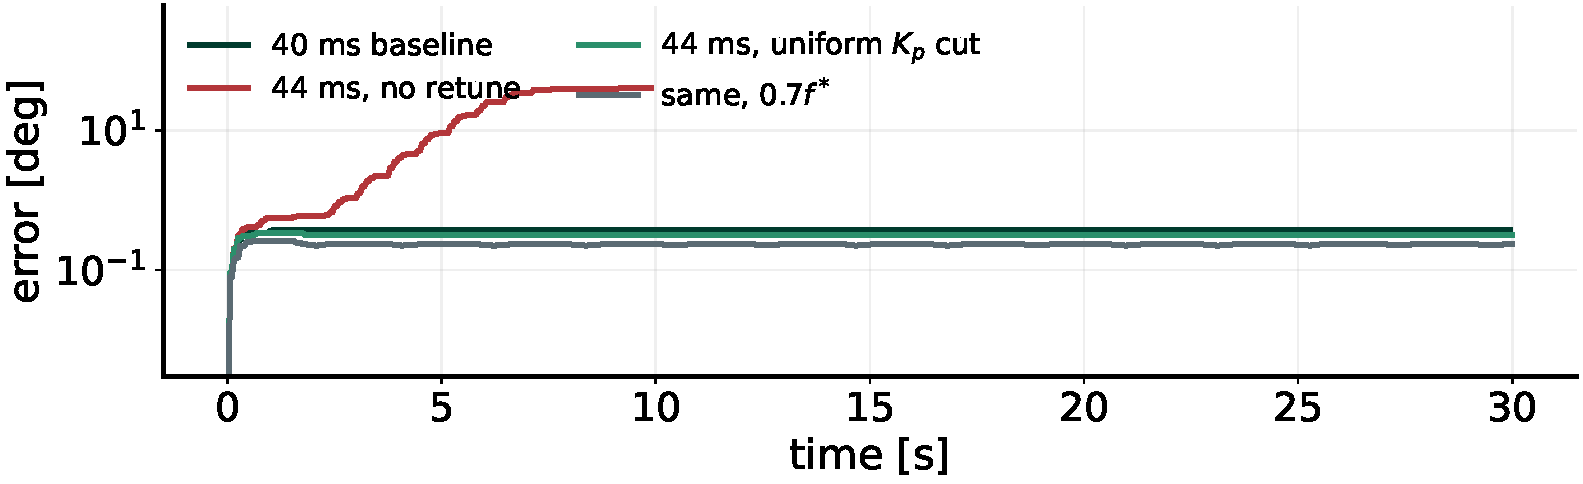
\includegraphics[width=268mm,height=82mm,keepaspectratio]{generated/figures/forced.pdf}\par
    {\fontsize{20pt}{23pt}\selectfont Forced response, 5 MW at bus 29, $f^{*}=4.65$ Hz (Julia, exact delay).\par}
    \vspace{0.5mm}
    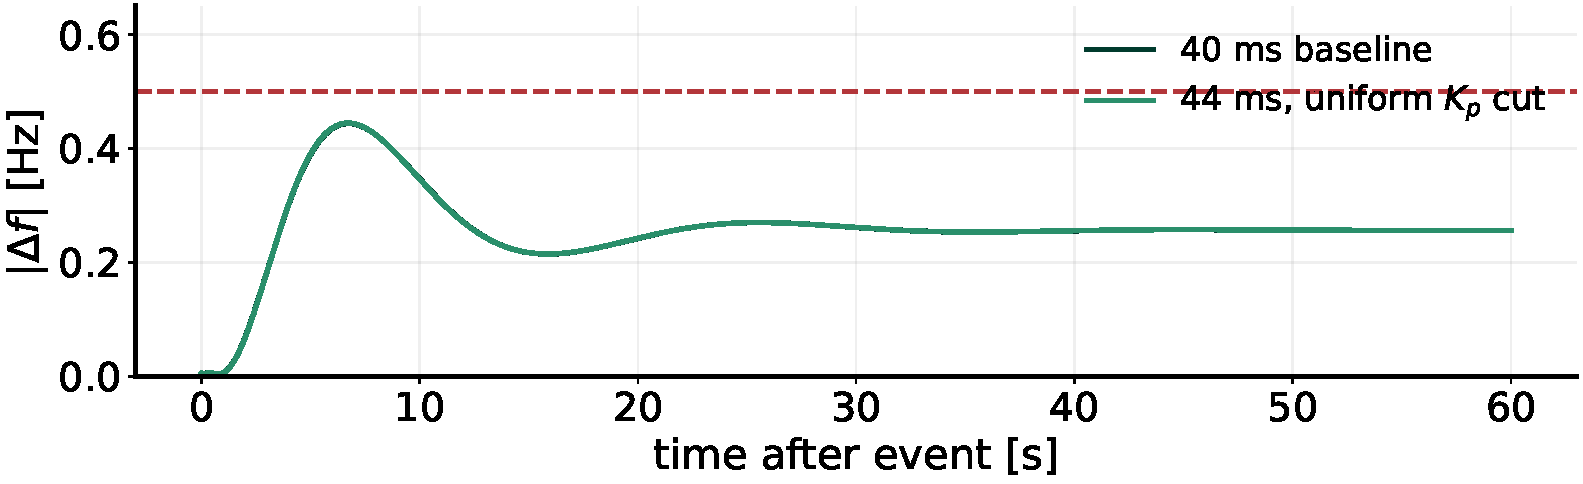
\includegraphics[width=268mm,height=82mm,keepaspectratio]{generated/figures/traj_events.pdf}\par
    {\fontsize{20pt}{23pt}\selectfont Load step $+100$ MW at bus 16: max bus-frequency deviation.\par}
    \vspace{0.5mm}
    {\fontsize{20pt}{23pt}\selectfont
    \begin{tabular}{@{}lccc@{}}
      \textbf{design} & \textbf{events} & \textbf{max $|\Delta f|$} & \textbf{slack}\\\hline
      baseline, 40 ms & 5/5 & 0.471 & 0.0074\\
      uniform $K_p$ $-14\,\%$, 44 ms & 5/5 & 0.472 & 0.0072\\
      6-site sparse, 44 ms & 4/5 & 0.492 & 0.0014\\
      no retune, 44 ms & abort & -- & --\\
    \end{tabular}\par}
    \vspace{0.5mm}
    {\fontsize{20pt}{23pt}\selectfont \textbf{Limits.} Floating-point counts, not certified; four-site retuning and the reduced-model 7--8 Hz family were refuted; five events are a finite campaign.\par}

    \vspace{2mm}
    \begin{tcolorbox}[colback=IASPaleGold,colframe=IASGold,boxrule=0.8pt,arc=1.5mm,left=2mm,right=2mm,top=1mm,bottom=1mm]
      {\fontsize{21pt}{25pt}\selectfont\textbf{TAKE-HOME} The closure is local (cycle 35--36, strongest couplings); the repair is global (one common $K_p$ cut). Sparse retuning of the core did not work in the full grid.\par}
    \end{tcolorbox}

  \end{PosterPanel}
\end{minipage}%
